\section{實驗}
本研究將真實度模型放在 Apache Spark 叢集當中運行,並且實際應用在串流XML文件上面。因串流資料講求即時接收即時處理,所以難在短時間內做真實度驗證。所以此模型使用在串流資料的環境下可以解決這樣的問題。本研究利用Open Data 所提供的XML自行撰寫資料產生器以及使用第三方XML文件產生器\cite{xmlgen}來產生XML文件,且每一個文件的大小皆不相同,實驗會使用客戶端程式隨機挑選文件進行上傳至串流伺服器,再由伺服器分別做資料前處理以及真實度計分,並且產生報表。\\\par
\subsection{真實度模型之串流XML文件應用架構}
本研究設計並實作真實度模型在 Apache Spark 叢集當中。Apache Spark 作為真實度計分伺服器,將接收來自客戶端傳送過來的資料,客戶端會使用 socket 將每一份XML 文件上傳至伺服器端。在Apache Spark 是使用 Spark Streaming 當中的 Socket streaming 來進行接收。而在 Socket streaming 當中會將接收到的資料進行處理,再由真實度模型進行計分,以下將針對系統當中的傳送端、處理模組以及真實度計分模組做介紹。\\\par

在資料傳送端,本研究自行實作Socket客戶端進行資料的上傳,每一個檔案會以字串的形式來做上傳,也就是說實際上客戶端發送的是持續產生的字串流,整體發送的時序圖如圖\ref{dataflow}所示:
\begin{figure}[H]
\centering
\graphicspath{{/Users/FUDA/Documents/masterThesis/image/}}
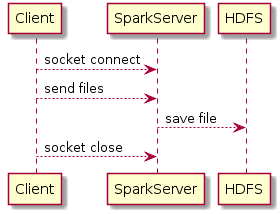
\includegraphics[scale=0.8]{dataflow.png}
\caption{資料接收與儲存流程}
\label{dataflow}
\end{figure}

在伺服器的處理模組使用的是Spark Streaming 來接收串流資料, 接收到串流資料的時候因資料是以字串流的方式發送的,所以資料處理模組會將字串流切分出每一個XML檔案,並且將處理過的資料直接送往真實度模型進行計算。資料傳送處理流程如圖\ref{recv}所示:
\begin{figure}[H]
\centering
\graphicspath{{/Users/FUDA/Documents/masterThesis/image/}}
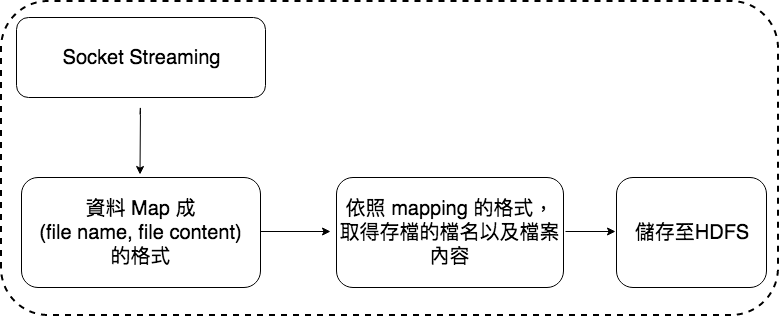
\includegraphics[scale=0.5]{recv.png}
\caption{資料傳輸處理模組}
\label{recv}
\end{figure}
資料傳送至真實度模型將傳送進來的XML文件與系統當中的基準文件做真實度計分,流程如圖\ref{process}所示:
\begin{figure}[H]
\centering
\graphicspath{{/Users/FUDA/Documents/masterThesis/image/}}
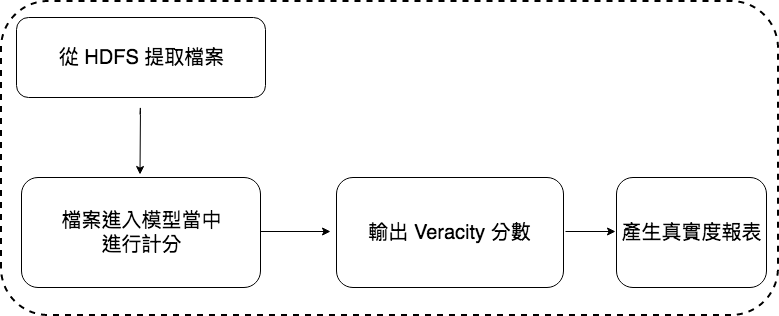
\includegraphics[scale=0.5]{process.png}
\caption{資料真實度計分模組}
\label{process}
\end{figure}

整體系統由傳送端、資料處理模組以及真實度模型計分模組所構成。利用串流做資料的上傳,從串流資料當中分割出每一個檔案來做儲存,並且使用真實度模型給予每一個檔案做真實度計分。完整系統架構如圖\ref{system}所示:
\begin{figure}[H]
\centering
\graphicspath{{/Users/FUDA/Documents/masterThesis/image/}}
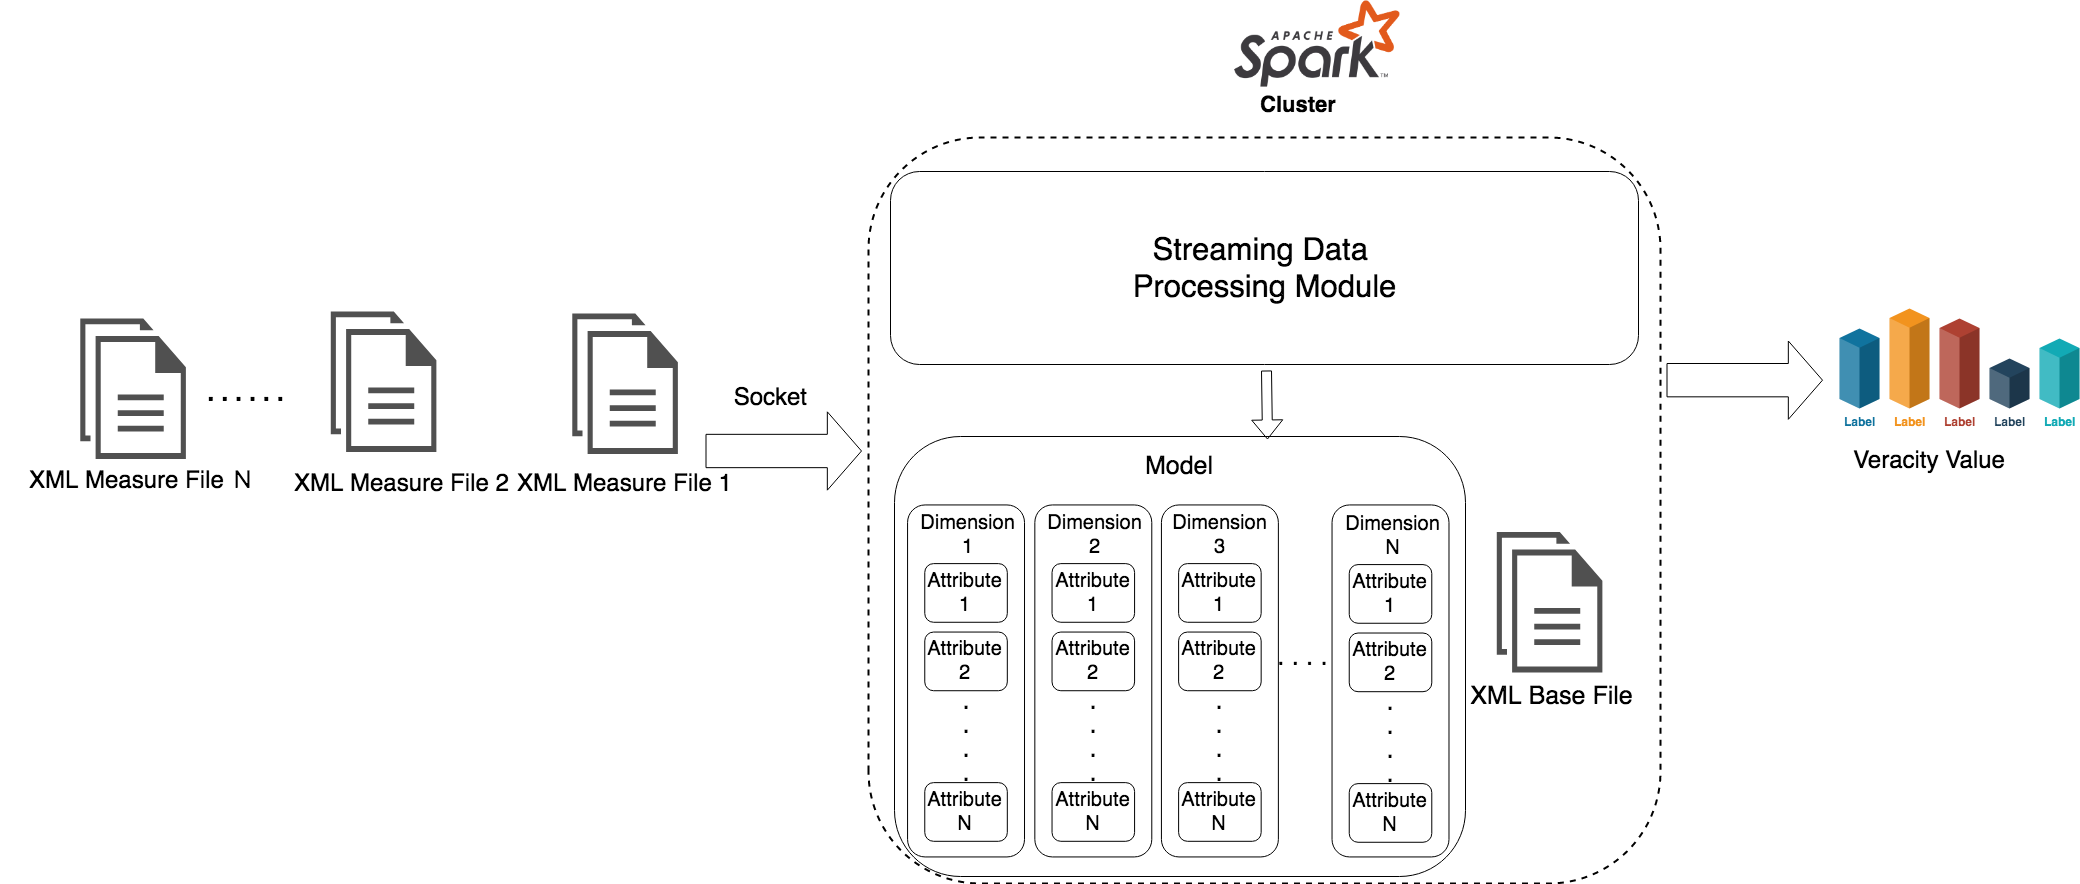
\includegraphics[scale=0.2]{streamingPro.png}
\caption{系統架構圖}
\label{system}
\end{figure}
\newpage
\subsection{真實度模型之應用實例}
本研究設計之真實度模型API應用在前面所提到的串流XML文件上,藉由實驗,驗證真實度模型應用於串流XML文件的可行性。而由於真實度的計算方式可彈性由使用者自行設計,所以根據前面的抽象類別,在真實度模型的設計應用上,本實驗設計了三個維度的真實度模型作為計算XML真實度的應用範例。\\\par
實驗設計的XML資料真實度應用範例具有三個維度,分別是文件節構、文件內容以及相似度。文件結構的維度當中有文件深度、節點數量兩個屬性,文件內容的維度當中有節點名稱以及路徑數量等兩個屬性,相似度的維度當中有路徑相似度以及節點名稱相似度兩個屬性。圖\ref{veracitymodel}為設計的模型架構:
\begin{figure}[H]
\centering
\graphicspath{{/Users/FUDA/Documents/masterThesis/image/}}
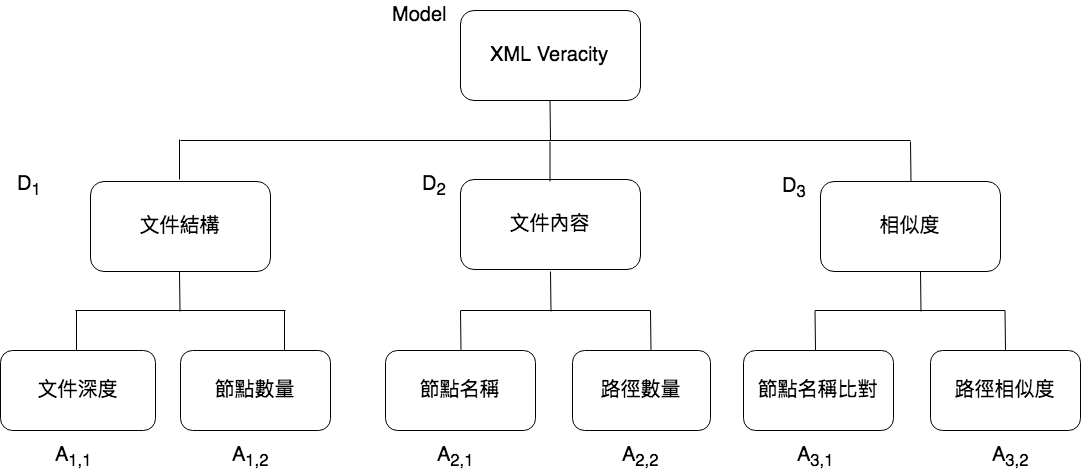
\includegraphics[scale=0.4]{xmlVeracity.png}
\caption{真實度模型}
\label{veracitymodel}
\end{figure}

這樣的架構可以對應到前面所提到的理論模型,在維度方面的定義$D_1$為XML文件結構,$D_2$為XML文件內容,$D_3$為相似度:
$$
M=\{D_1,\ D_2,\ D_3\}\\
$$
在$D_1$維度下會有2個屬性$A_{1,1}$和$A_{1,2}$,$A_{1,1}$為文件深度,$A_{1,2}$為節點數量:
$$
D_1=\{A_{1,1},\ A_{1,2}\}\\
$$
而在$D_2$維度下會有2個屬性$A_{2,1}$以及$A_{2,2}$。而屬性$A_{2,1}$代表節點名稱,$A_{2,2}$代表路徑數量:
$$
D_2=\{A_{2,1},\ A_{2,2}\}\\
$$
在$D_3$維度下有兩個屬性,$A_{3,1}$和$A_{3,2}$,分別代表節點名稱比對以及路徑相似度\cite{ristad1998learning},路徑相似度的作法是借鏡編輯距離,編輯距離會計算從字串A變成字串B需要經歷多少次的新增刪除修改,而路徑的相似度則去計算要從路徑A變成路徑B需要經歷過多次的新增刪除修改:
$$
D_3=\{A_{3,1},\ A_{3,2}\}\\
$$
理論模型確立之後,即可以依照這樣的架構來實作模型,模型建立的演算法如圖\ref{createmodel}所示:
\begin{figure}[H]
\centering
\graphicspath{{/Users/FUDA/Documents/masterThesis/image/}}
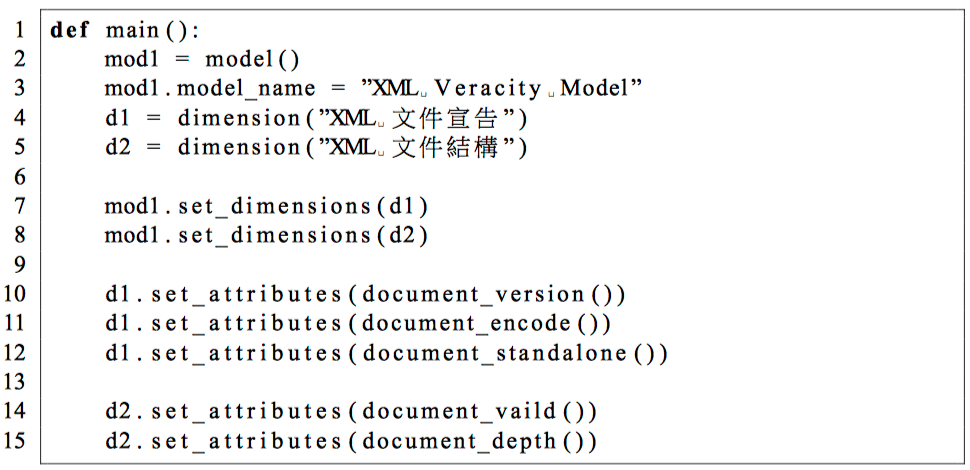
\includegraphics[scale=0.36]{createModel.png}
\caption{模型建立演算法}
\label{createmodel}
\end{figure}
接者需要設計每一個屬性的計分方式(Quantification)。而三個維度的計分方式都基於Dataguides\cite{oem}\cite{dataguides}\cite{oemweb}的結構做比較所謂的Dataguides是一種將XML的樹狀結構進行精簡化,來加速XML查詢以及節點走訪的速度,並且還可以保留各節點之間的關係。以文件結構的維度來說,下面兩個屬性:文件深度以及節點數量,在文件深度來說如果兩棵樹深度相同。在系統計分上會為滿分,如果被量測文件的樹深度與基準文件相差2以內,則分數會照著比例增加。比方說基準文件深度為5,如果被量測文件的深度為6或是4,那分數的就為加20\%。如果深度的差距到達了2層以上,系統即認為被量測文件與基準文件的資訊差異過大,所以會以比例開始扣分。在節點數量方面,如果被量測文件與基準文件的節點總數相差5個以內 ,系統會認為真實程度高,分數會較為高分。而節點數相差5個到10個以內,系統計分會偏低分。而大於10個以上則為不及格分。\\\par

在文件內容的維度來說,在節點名稱的屬性中,系統會從基準文件中隨機挑選五個節點,並且去比較在被量測文件中是否有這五個節點,有的話則依比例給分。在路徑數量的屬性中,會依照Dataguides所擷取出來的路徑數量為依據,來比較基準文件與被量測文件的路徑數量,並且依照被量測文件與基準文件的路徑數量一比例計分。\\\par

在相似度的的維度裡面,計算方法會使用常聽到的編輯距離相似度計算\cite{ristad1998learning}的方式來評分,路徑相似度的部分,系統會將基準文件與被量測文件中的最長路徑提取出來,進行編輯距離相似度比較,計算出來的相似度分數再乘上100即為屬性分數。在節點名稱比對的部分,系統會從基準文件隨機挑選五個節點,並且比較被量測文件中是否擁有這五個節點,如果有的話則依比例加分。

\subsection{實驗環境}
實驗環境是使用三台實體電腦。作業系統為Linux 發行版 Ubuntu 16.04 LTS,使用之CPU皆為8 核心,master 為16GB記憶體,兩台slave記憶體為12GB。表\ref{cluster}為機器的詳細規格。使用之Hadoop 版本為2.7,Spark版本為2.0。在HDFS中我們將每一個區塊的資料副本設置為3,軟體環境配置如表\ref{software}。
\begin{table}[H]
\begin{center}
\caption{叢集電腦規格}
\label{cluster}
\begin{tabular}{|p{3cm}<{\centering}|p{3cm}<{\centering}|p{3cm}<{\centering}|}
\hline
&Master 1台&Slave 2台\\
\hline
OS&Ubuntu 16.04 LTS&Ubuntu 16.04 LTS\\
\hline
CPU&Intel Core i7 8700@2.93GHz&Intel(R) Xeon(R) CPU E3-1230 v3 @ 3.30GHz\\
\hline
核心數&8&8\\
\hline
Memory&32 GB&12 GB\\
\hline
儲存空間&500 GB&1 TB\\
\hline
\end{tabular}
\end{center}
\end{table}

\begin{table}[H]
\caption{使用軟體版本}
\label{software}
\begin{center}
\begin{tabular}{|p{3cm}<{\centering}|p{3cm}<{\centering}|}
\hline
軟體名稱 & 版本號\\
\hline
Hadoop & 2.7版\\
\hline
Apache Spark &2.0版\\
\hline
Python & 3.6版\\
\hline
\end{tabular}
\end{center}
\end{table}

\newpage
\subsection{實驗設計}
實驗主要分成三個部分,主要的目的是要展現真實度模型的可用性以及確認在Apache Spark 中達到的平行化運算的效果。為了展現模型的效果,在第一部分的實驗中設計了一個Dashboard,用以觀察真實度模型的計分以及可視化串流文件計分的結果。第二部分則是從Apache Spark 所提供的 Web UI介面觀察資料在平行化運算的狀況,以確認對於傳流文件的處理是否有達到平行化加速的作用。第三部分的實驗將準備三種不同種類的XML文件,並且使用XML文件產生器將文件的結構做延展以及依照三種不同XML文件的規則來產生文件。在傳送的時候將三種不同種類文件混合在一起傳送,觀察真實度模型是否能正確的進行計分,並且將混合傳送的文件計算真實度並且做出三種分類。\\\par

\subsection{實驗結果}
第一部分為資料Dashboard,Dashboard的創建是使用Dash\cite{dash},Dash為一個開源的DashBoard軟體,可以自定義版面以及資料呈現方式。在Dashboard當中設計有兩個圖表,雷達圖以及表格。第一種雷達圖用來顯示真實度模型所計算出來的真實度計分,使用雷達圖上表示的面積計算出來的真實度,根據面積大小,使用者可以直接觀察到真實度的變化,Dashboard的雷達圖所呈現的真實度如圖\ref{radarchart}所示。
\begin{figure}[H]
\centering
\graphicspath{{/Users/FUDA/Documents/masterThesis/image/}}
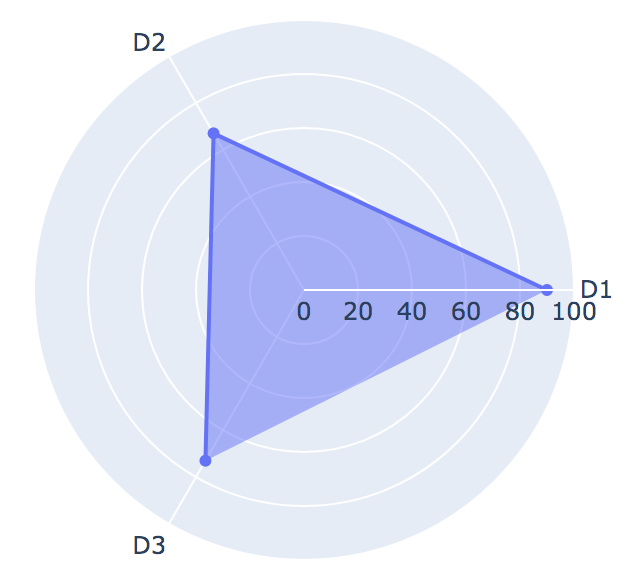
\includegraphics[scale=0.6]{radarchart.png}
\caption{真實度雷達圖}
\label{radarchart}
\end{figure}

在圖\ref{radarchart}當中,可以觀察到真實度模型的三個維度的計分。$D_1$的分數接近90分,$D_2$的分數大約為70分,$D_3$的分數約接近80。由這樣的觀察可以發現這份被量測文件的真實程度很高。\\\par
第二種表格呈現則是將真實度模型當中每一個屬性、維度以及最後的總分做完整的呈現,以補足雷達圖無法表達的細節,表格的節錄呈現如圖\ref{veracitytable}所示:
\begin{figure}[H]
\centering
\graphicspath{{/Users/FUDA/Documents/masterThesis/image/}}
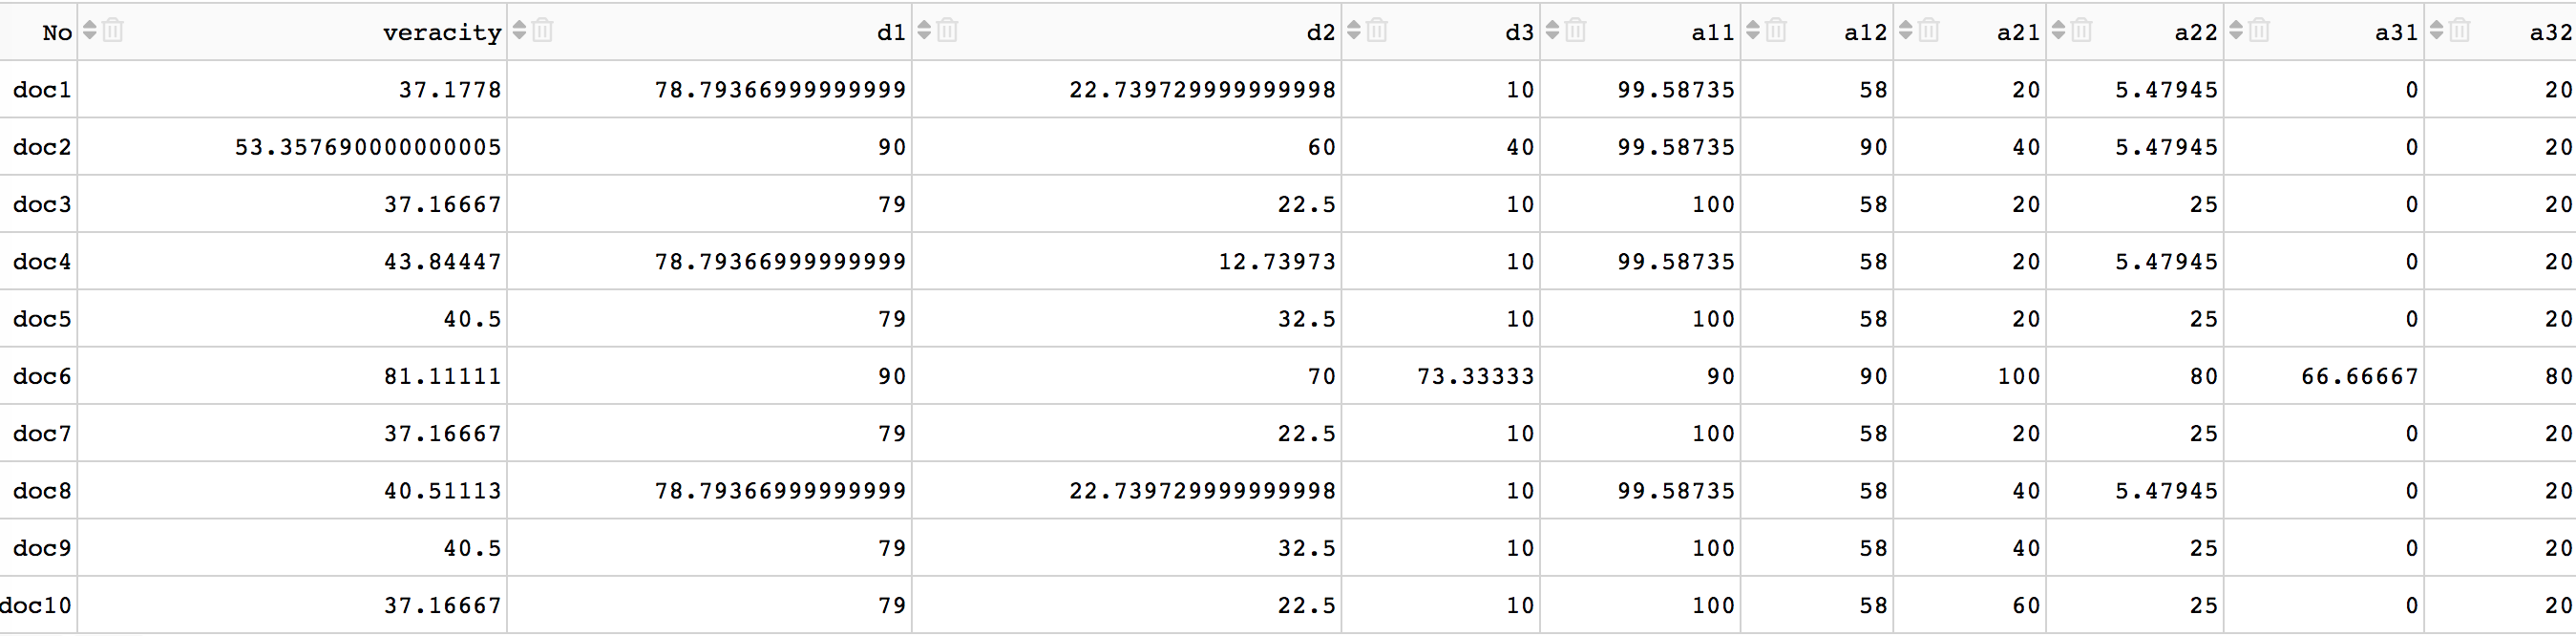
\includegraphics[scale=0.37]{veracitytable.png}
\caption{真實度表格節錄}
\label{veracitytable}
\end{figure}
在圖\ref{veracitytable}當中可以看到有著每一份被量測文件的文件編號、屬性分數、維度分數以及最後的真實度計分。在前面的雷達圖當中所呈現的是三個維度的面積,而在表格當中是呈現詳細的數據。使用者可以做交叉比對,來驗證每一份XML的真實程度。\\\par
第二部分的實驗會從Apache Spark 所提供的Web UI當中觀察串流資料的平行化,已確認串流資料的平行化。圖\ref{sparkcompute}為Apache Spark 所提供的Web UI,在當中有三列,分別代表著三台主機,而其中一欄為Active Tasks,代表說有幾幾個任務在主機上面運行,可以從圖中得知Spark driver 有將任務分發到兩台slave 去做計算,可以看到兩台slave的Active Tasks 數量都各為1,所以可以驗證平行化運算是有效的。
\begin{figure}[H]
\centering
\graphicspath{{/Users/FUDA/Documents/masterThesis/image/}}
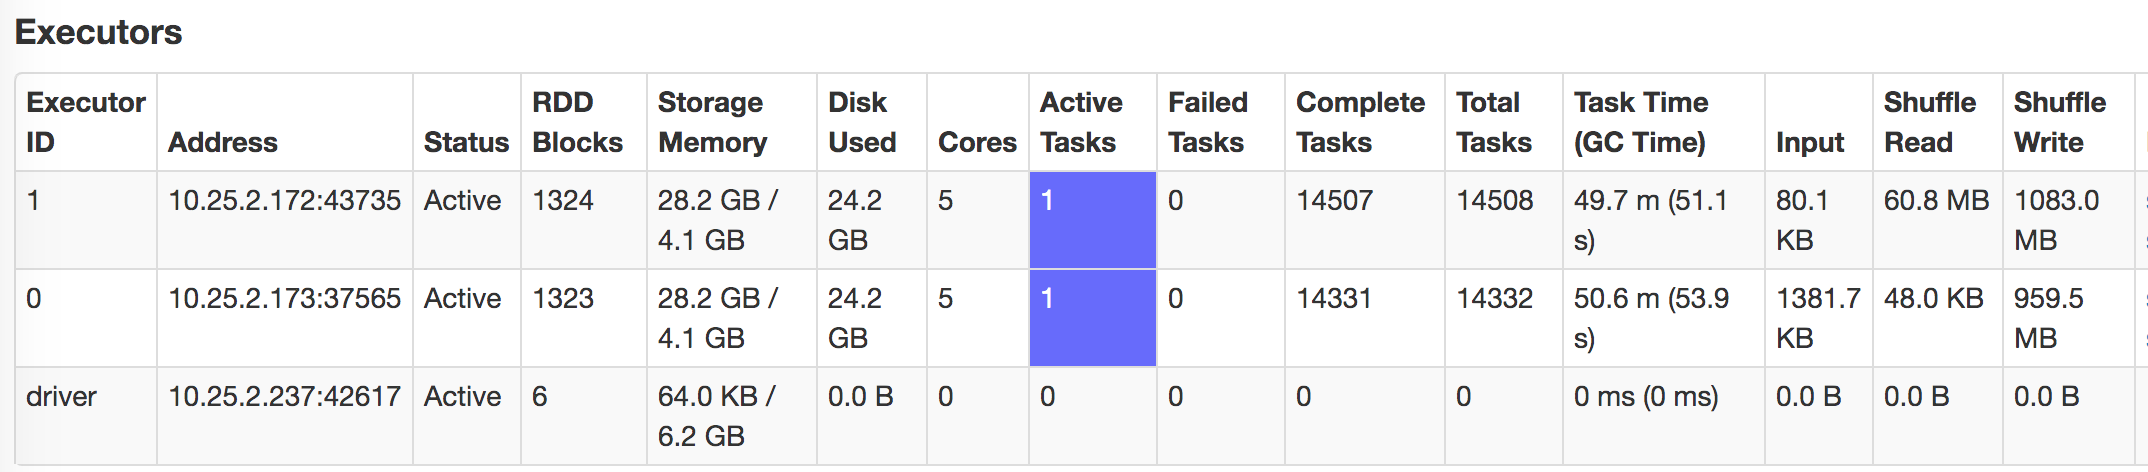
\includegraphics[scale=0.45]{sparkcompute.png}
\caption{Apache Spark 平行化}
\label{sparkcompute}
\end{figure}
最後一部分為實驗真實度模型能否將混合傳輸的資料分出不同的真實度, 實驗中準備了三種種類的XML文件,分別是美國的郵遞區號資料集\cite{usazipcode}、世界氣象的資料集\cite{worldweather}以及XML產生器所產生出來的資料集。郵遞區號的資料集Dataguides如圖\ref{zipcode.dot}所示,而世界氣象的資料集所產生出來的Dataguides如\ref{weather.dot}所示:
\begin{figure}[H]
\centering
\graphicspath{{/Users/FUDA/Documents/masterThesis/image/}}
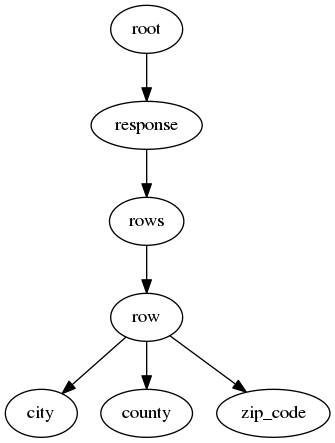
\includegraphics[scale=0.7]{zipcode.png}
\caption{郵遞區號資料集Dataguides}
\label{zipcode.dot}
\end{figure}

\begin{figure}[H]
\centering
\graphicspath{{/Users/FUDA/Documents/masterThesis/image/}}
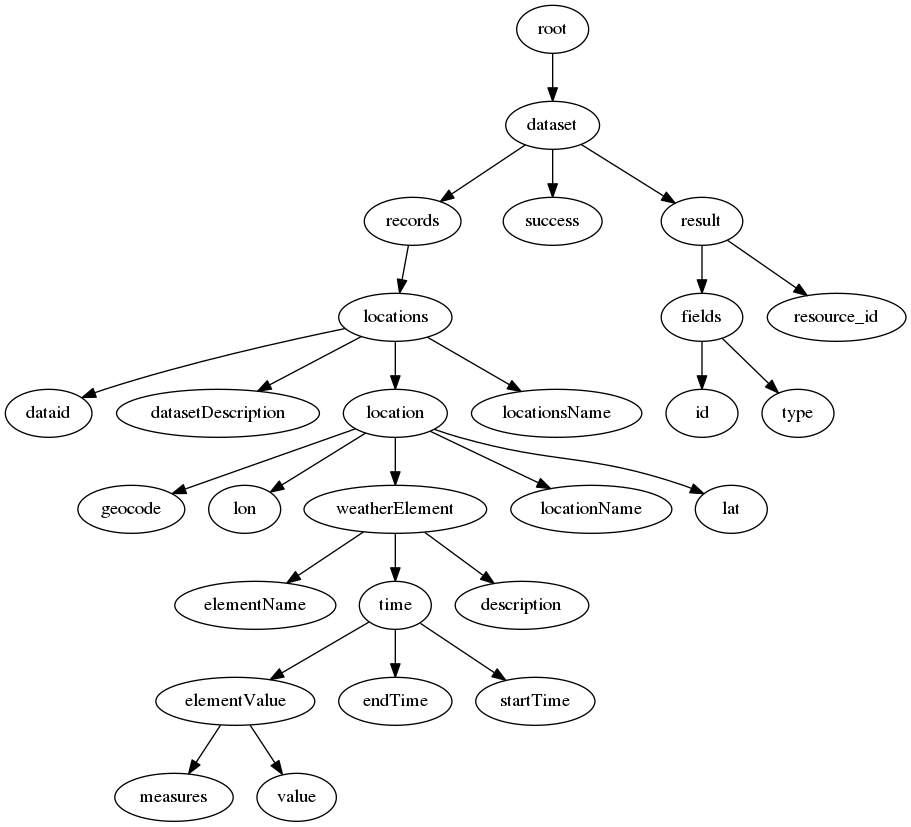
\includegraphics[scale=0.5]{weather.png}
\caption{世界天氣資料集Dataguides}
\label{weather.dot}
\end{figure}

實驗中將利用圖\ref{zipcode.dot}以及圖\ref{weather.dot}的架構撰寫文件產生器,以產生不同大小的文件來進行實驗,實驗將分成,三次實驗分別會更換三種基準文件,來測試真實度模型是否能依照基準文件來分類真實度不同的XML文件。\\\par
第一次實驗將美國郵遞區號資料集作為基準文件,第二次實驗將使用世界天氣資料集作為基準文件,第三次實驗將使用第三方XML產生器所產出的文件作為基準文件,並且比較三次實驗的平均真實度計分。\\\par

表\ref{zipbase}為第一次實驗的結果,可以從真實度計分觀察到基準文件與被量測文件同為美國郵遞區號資料集的時候,真實程度有80分以上,不同種類的資料及真實程度都明顯較低,分數都落在40分以下,可以證明模型有能力將不同種類的文件分類出來。
\begin{table}[H]
\begin{center}
\caption{基準文件為美國郵遞區號的真實度評分}
\label{zipbase}
\begin{tabular}{|p{3cm}<{\centering}|p{2.5cm}<{\centering}|p{2cm}<{\centering}|p{2cm}<{\centering}|p{2cm}<{\centering}|}
\hline
文件種類& $D_1$ &$D_2$ &$D_3$ & 真實度計分 \\
\hline
美國郵遞區號&90&78&73.33333 &80.9444438\\
\hline
世界天氣&79&29.16666667&10 &39.6582491\\
\hline
文件產生器 &78.79367&20.21486182&10&35.3597464\\
\hline
\end{tabular}
\end{center}
\end{table}
表\ref{weatherbase}為第二次實驗結果,基準文件使用世界天氣資料集,可以觀察到世界天氣的被量測文件獲得了96分,表示模型可以成功將此一種類的資料真實度分類出來。其他種類的資料真實程度也都明顯低落,分數都落在50分以下。
\begin{table}[H]
\begin{center}
\caption{基準文件為世界天氣的真實度評分}
\label{weatherbase}
\begin{tabular}{|p{3cm}<{\centering}|p{2.5cm}<{\centering}|p{2cm}<{\centering}|p{2cm}<{\centering}|p{2cm}<{\centering}|}
\hline
文件種類& $D_1$ &$D_2$ &$D_3$ & 真實度計分 \\
\hline
美國郵遞區號&74&16.7&3.125 &31.2416678\\
\hline
世界天氣&94.79&96.20625&99.03125 &96.60917\\
\hline
文件產生器&78.79367&21.18450232&9.375 &36.45106141\\
\hline
\end{tabular}
\end{center}
\end{table}
最後一個實驗的實驗結果為表\ref{docbase},基準文件為XML產生器所產生的文件,可以從表中觀察到真實度模型也可以成功將這類型的文件分類出來,並且還可以觀察到文件產生器的分數幾乎接近滿分,其原因為此類的資料是使用產生器所產生的,因為有一定的產生規則,所以導致每一份被量測文件與基準文件的差異過小,導致比對的時候真實程度差異不大。
\begin{table}[H]
\begin{center}
\caption{基準文件為文件產生器所產生之文件的真實度評分}
\label{docbase}
\begin{tabular}{|p{3cm}<{\centering}|p{2.5cm}<{\centering}|p{2cm}<{\centering}|p{2cm}<{\centering}|p{2cm}<{\centering}|}
\hline
文件種類& $D_1$ &$D_2$ &$D_3$  & 真實度計分\\
\hline
美國郵遞區號&29.13736	&3.15479&0.67568 &10.9226099	\\
\hline   
世界天氣&29.20633&13.68617273&2.02703 &14.70382\\
\hline
文件產生器&100&99.99293887&100 &99.99764629\\
\hline
\end{tabular}
\end{center}
\end{table}
綜合以上三次實驗可以觀察到三種種類的XML文件皆可以用真實度模型進行分類,其真實程度可以完全區分出三種不同的XML,從三次實驗的數據可以觀察到文件真實度分數的鑑別度,驗證了模型的可行性。